\subsection{Impact of Analytic Traffic Characteristics}\label{sec:network:performance_model:numerical_examples}
First, we validate our performance model by comparing the analytical results with simulations based on measured
packet traces of two real smartphone applications .
Then, we investigate the impact of traffic patterns on signalling load and power drain and derive high-level implications of the model.

\subsubsection*{Model Validations}\label{sec:network:performance_model:validations}

In order to assess the applicability of our performance model, we first have to check whether real-world application traces can be modeled as renewal process, which was our main assumption for the model.
We use the Lewis-Robinson-Test \cite{Ascher1984}, which is a hypothesis test with null hypothesis \(H_0\) that the tested process is a renewal process.
To this end, we use exemplary the measurement, obtained with the measurement testbed introduced in \refsec{sec:network:network_traces:performance_evaluation:measurement}, for two different types of applications: \emph{Twitter} and \emph{K9-Mail}.
According to this test, the null hypothesis cannot be rejected for both of our packet traces at a significance level of \SI{95}{\percent}.
Although this assumption may not be true for all applications, our results show that at least the considered applications can be modeled as a renewal process.

Next, we compare our analytical performance results with \gls{RRC} protocol simulations using measured application and \gls{TCP} traces which are described in more detail in \refsec{sec:network:network_traces:numerical_results:traffic_characterization}.
In order to produce analytical results that correspond to the real applications, we extract the empirical distributions of the inter-packet time \(\PacketIAT\) from the traces for both applications and use these distributions as input for \refeq{eq:network:performance_model:system_description:state_distribution:observation_density}. 

In \reffig{fig:network:performance_model:numerical_examples:validations:analytic_vs_simulation} we compare the accuracy of the results  obtained by the presented method to the values obtained from simulations for the two measured applications and both considered metrics.
We observe that the accuracy for both power drain \(\gls{PD}\) and \(\gls{SI}\) is very high.
In \reffig{fig:network:performance_model:numerical_examples:validations:analytic_vs_simulation:signalling_intensity} the results for both the Mail and Twitter application obtained by the model completely align with the signalling intensity obtained by the simulation.
The comparison of analytical results for the power drain to the simulation in \reffig{fig:network:performance_model:numerical_examples:validations:analytic_vs_simulation:power_drain} leads to the same conclusions as for the signalling intensity.

\begin{figure}
	\begin{subfigure}[b]{\textwidth}
	\centering
	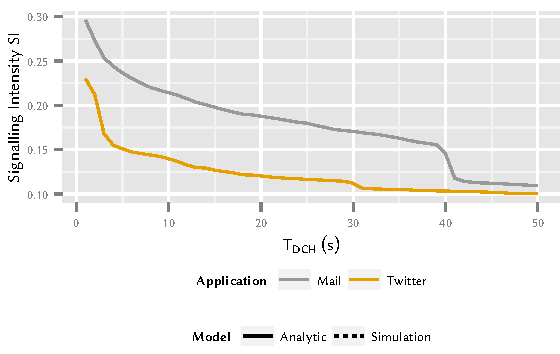
\includegraphics{network/performance_model/numerical_examples/figures/3state_tdch_si_analytic_simulative}
	\caption{Signalling intensity}\label{fig:network:performance_model:numerical_examples:validations:analytic_vs_simulation:signalling_intensity}
	\end{subfigure}

	\begin{subfigure}[b]{\textwidth}
	\centering
	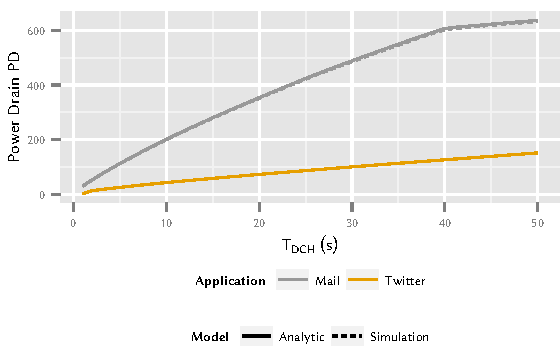
\includegraphics{network/performance_model/numerical_examples/figures/3state_tdch_pd_analytic_simulative}
	\caption{Power drain}\label{fig:network:performance_model:numerical_examples:validations:analytic_vs_simulation:power_drain}
	\end{subfigure}

	\caption{Comparison of the performance model with a \headershortacr{3G} simulation for the Three State Scenario. Lines overlap due to good fit.}\label{fig:network:performance_model:numerical_examples:validations:analytic_vs_simulation}
\end{figure}

\subsubsection*{Impact of Traffic Patterns on Signalling Intensity}\label{sec:network:performance_model:signalling_intensity}
First, we focus on the signalling intensity \(\gls{SI}\) of traffic patterns and check the impact of the average inter-packet time \(E[\PacketIAT]\) and the timer configuration. The signalling intensity \(\gls{SI}\), i.e., the average number of state transitions required for the transmission of a single packet, is an abstract measure for the signalling load produced by a specific traffic pattern.

\paragraph*{Impact of the Average Inter-Packet Time \(E[\PacketIAT]\)}\label{sec:network:performance_model:signalling_intensity:ea}
Some applications, for example those downloading or streaming of videos, send and receive large amounts of data within short time frames.
In contrast, other applications, e.g. social network clients send and receive small amounts of data every few minutes over the time span of some hours or days.

In this section we study the impact of average inter-packet times \(E[\PacketIAT]\) and the burstiness of the traffic pattern, i.e., the coefficient of variation 
\[c_{\PacketIAT} = \frac{\sqrt{\mathrm{Var}[\PacketIAT]}}{\mathrm{E}[\PacketIAT]}\]
 on the signalling load.
For that purpose, we use the simple Two State Model, set the timer \(\gls{TDCH}=\SI{10}{\second}\), consider only the first and the second moment of the inter-packet time \(\PacketIAT\), and assume that \(\PacketIAT\) follows a log-normal distribution, where both moments can be varied independently.

\begin{figure}
	\centering
	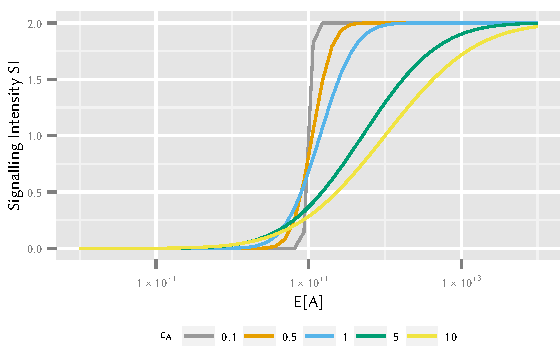
\includegraphics{network/performance_model/numerical_examples/figures/2state_ea_si}
	\caption{Signalling intensity \gls{SI} for different traffic patterns considering the Two State Model with \(\headershortacr{TDCH}=\SI{10}{\second}\) for different traffic patterns.}
	\label{fig:network:performance_model:numerical_examples:validations:analytic_vs_simulation:2state_ea_si}
\end{figure}

In \reffig{fig:network:performance_model:numerical_examples:validations:analytic_vs_simulation:2state_ea_si}, we vary the average inter-packet time \(E[\PacketIAT]\) in six orders of magnitude and investigate the resulting signalling intensity \(\gls{SI}\) for different coefficients of variation \(c_{\PacketIAT}\).
We observe that \(c_{\PacketIAT}\) has no impact on \(\gls{SI}\) for very small inter-packet times \(E[\PacketIAT]<\SI{1e-1}{\second}\).
Here, the \gls{UE} stays in state \gls{RRC_DCH} for the complete time since no inter-packet times \(\PacketIAT>\gls{TDCH}\) occur.
In addition, the impact of \(c_{\PacketIAT}\) is small for very large values of \(E[\PacketIAT]>\SI{1e3}{\second}\).
In this case, the \gls{UE} switches to state \gls{RRC_DCH} and back to state \gls{RRC_idle} for the transmission of every packet. Therefore, the signalling intensity \(\gls{SI}\) approaches the value 2.
For values in between these two extremes, the coefficient of variation \(c_{\PacketIAT}\) has a considerable impact on the signalling intensity \(\gls{SI}\).
More periodic traffic, i.e. smaller values of \(c_{\PacketIAT}\), results in an increase of \(\gls{SI}\) from 0 to 2 very sharp at the value \(E[\PacketIAT]=\gls{TDCH}\), while this increase is more smooth for larger values of \(c_{\PacketIAT}\).
This is due to the fact that for nearly periodic traffic it is crucial whether the timer value \(\gls{TDCH}\) is smaller or larger than \(E[\PacketIAT]\). 
For larger values of \(c_{\PacketIAT}\) this dependency is weaker.

\paragraph*{Impact of the Coefficient of Variation of the Inter-Packet Time \(c_\PacketIAT\)}

Next, we focus on the impact of the timer value \(\gls{TDCH}\) with respect to the burstiness of the traffic.
We use the same setting as before, but fix the average inter-packet time \(E[\PacketIAT]=\SI{4}{\second}\).
While there are differences in \(E[\PacketIAT]\) among users in real world settings, measurement studies have revealed that across all users \(\SI{95}{\percent}\) of the packets are received or transmitted within \(\SI{4.5}{\second}\) of the previous packet \cite{Falaki2010a}.
Therefore, the order of magnitude of \(E[\PacketIAT]=\SI{4}{\second}\) is of practical relevance. 

\begin{figure}
	\centering
	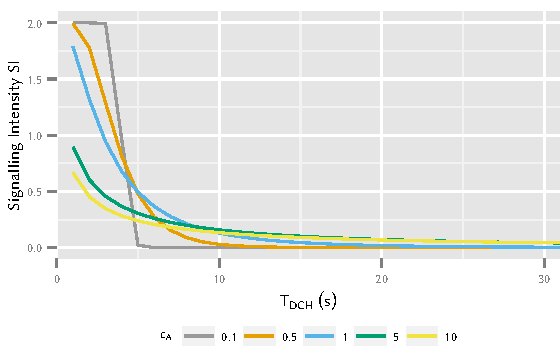
\includegraphics{network/performance_model/numerical_examples/figures/2state_tdch_si}
	\caption{Signalling intensity \(\headershortacr{SI}\) for the Two State Model w.r.t. different timeout values \(\headershortacr{TDCH}\) and coefficient of variations \(c_{\PacketIAT}\).}
	\label{fig:network:performance_model:numerical_examples:validations:analytic_vs_simulation:2state_tdch_si}
\end{figure}


The signalling intensity \(\gls{SI}\) is shown in \reffig{fig:network:performance_model:numerical_examples:validations:analytic_vs_simulation:2state_tdch_si} with respect to the timer value \(\gls{TDCH}\) and the burstiness \(c_{\PacketIAT}\) of the traffic pattern.
Obviously, larger timers lead to less frequent state transitions and therefore to less signalling load.
We observe in addition that the impact of the timer is crucial for nearly periodic traffic.
If the average inter-packet time for nearly periodic traffic is larger than the timer, then every packet transmission involves a state transitions from \gls{RRC_idle} to \gls{RRC_DCH} and a transition back.
In contrast, no transitions are required if the average inter-packet time is shorter than the timer.
With increasing values of \(c_{\PacketIAT}\) the impact of the timer is reduced.
This means that for bursty traffic patterns the timer value is of less importance with respect to the generated signalling load.

\subsubsection*{Impact of Traffic Patterns on Power Drain of the \headershortacr{UE}}\label{sec:network:performance_model:power_drain}
In this section we study the impact of the traffic patterns on the power drain \(\gls{PD}\) of the \gls{UE}.
This metric quantifies how resource-efficient specific traffic patterns and timer configurations are for the battery of the \gls{UE}.

\begin{figure}
	\centering
	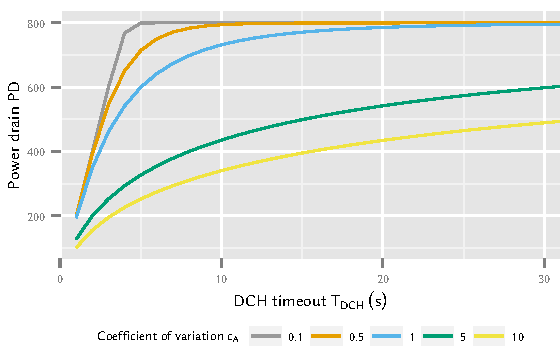
\includegraphics{network/performance_model/numerical_examples/figures/2state_tdch_pd}
	\caption{Power drain \(\headershortacr{PD}\) for the Two State Model w.r.t. different timeout values \(\headershortacr{TDCH}\) and coefficient of variations \(c_{\PacketIAT}\).}
	\label{fig:network:performance_model:numerical_examples:validations:analytic_vs_simulation:2state_tdch_pd}
\end{figure}

For the power drain in the different \gls{RRC} states, we use the same radio network power drain  used in \refsec{sec:network:network_traces:calculating_metrics}.
We investigate the impact of the average inter-packet time, the impact of the timer configuration and validate our model with simulations. 
In \refsec{sec:network:performance_model:signalling_intensity:ea} we have seen that no state transitions occur for very small and very large average inter-packet times \(E[\PacketIAT]\).
This was due to the fact that for very small values the \gls{UE} is continuously in state \gls{RRC_idle} and for large values it switches to state \gls{RRC_DCH} for every packet.
Thus, traffic patterns with very small and very large inter-packet times \(E[\PacketIAT]\) have also no impact on the power drain of the \gls{UE} regardless of the burstyness represented by the coefficient of variation \(c_{\PacketIAT}\).

To study the impact of the timer configuration \(\gls{TDCH}\), we use the same setting as for the signalling load: log-normal distribution of inter-packet time \(\PacketIAT\), \(E[\PacketIAT] = \SI{4}{\second}\) in the Two State Model.
The numerical values shown in \reffig{fig:network:performance_model:numerical_examples:validations:analytic_vs_simulation:2state_tdch_pd} indicate that longer timeouts lead to a higher power drain \(\gls{PD}\).
This is reasonable since the UE stays longer in the power intensive \gls{RRC_DCH} state in these cases.
However, we observe that the burstiness of the traffic pattern has also a considerable impact on the power drain \gls{PD}. 
For example, for \(\gls{TDCH} = \SI{15}{\second}\), the power drain is only \(\SI{400}{\milli\watt}\) for very bursty traffic with \(c_{\PacketIAT} = 10\), while it is almost \(\SI{400}{\milli\watt}\) for less bursty traffic with a \(c_{\PacketIAT} = 1\). 
The reason is that bursty traffic patterns send a lot of traffic during short periods when the UE is in state \gls{RRC_DCH} anyway. During the following off-periods that \gls{UE} can save power in \gls{RRC_idle} state.
Hence, we conclude that longer timeouts and smaller coefficients of variation \(c_{\PacketIAT} = 1\), i.e. more periodic and less bursty traffic, result in a higher power drain of the \gls{UE}.

\subsubsection*{Tradeoff: Energy Consumption vs. Signalling Load}\label{sec:network:performance_model:trade_off}
In \reffig{fig:network:performance_model:numerical_examples:validations:analytic_vs_simulation:2state_pd_vs_si_vs_tdch}, we show the effect of network parameter optimisation using the timer \gls{TDCH} on traffic patterns with varying coefficient of variation.

\begin{figure}
	\centering
	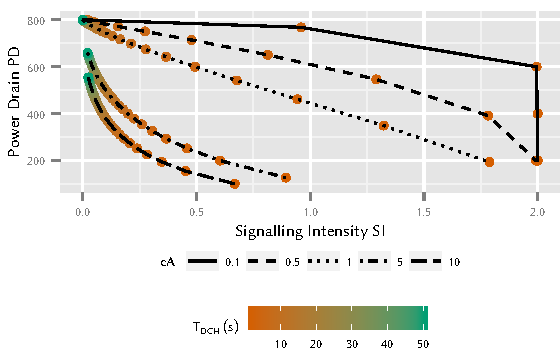
\includegraphics{network/performance_model/numerical_examples/figures/2state_pd_vs_si_vs_tdch}
	\caption{Trade-off between \(\headershortacr{PD}\) and \headershortacr{SI} for the Two State Model.}
	\label{fig:network:performance_model:numerical_examples:validations:analytic_vs_simulation:2state_pd_vs_si_vs_tdch}
\end{figure}

We see that optimisations may decrease signalling by large amounts while only having very little impact on power drain for one specific kind of traffic.
The same timer setting could increase the power drain for another kind of traffic while only offering little benefit with regard to the generated signalling intensity.